\documentclass{standalone}
\usepackage{tikz}
\usepackage{graphicx}
\usetikzlibrary{decorations.pathreplacing,angles,quotes}


\begin{document}

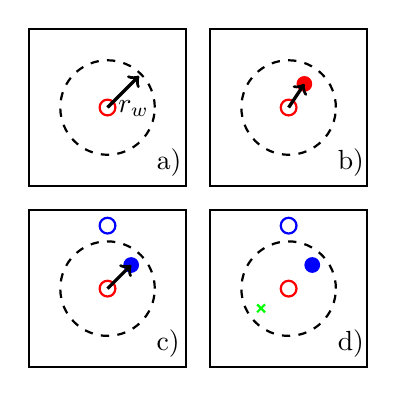
\begin{tikzpicture}
    % grid size
    \def \gs {10}

    %\draw [help lines] (-\gs,-\gs) grid (\gs,\gs);
    %Top Left
    \draw[thick] (0,0) rectangle (2,-2);
    \draw[red,thick] (1,-1) circle (0.1);
    \draw[thick,dashed] (1,-1) circle (0.6);
    \node[text width=5, right] at (1.5,-1.7) {a)};
    
    \draw[very thick] [->] (1,-1) -- (1.4,-0.6) node[below, xshift=-2, yshift=-5] {$r_w$};
      
    %Top Right
    \draw[thick] (2.3,0) rectangle (4.3,-2);
    \draw[red,thick] (3.3,-1) circle (0.1);
    \draw[thick,dashed] (3.3,-1) circle (0.6);
    \node[text width=5, right] at (3.8,-1.7) {b)};
    
    \fill[red!100] (3.5,-0.7) circle (0.1);
    \draw[very thick] [->] (3.3,-1) -- (3.5,-0.7);
    %\draw[red, very thick] [->] (4,-1) -- (4.3,-0.7);
    
    %Bot Left
    \draw[thick] (0,-2.3) rectangle (2,-4.3);
    \draw[red,thick] (1,-3.3) circle (0.1);
    \draw[thick,dashed] (1,-3.3) circle (0.6);
    \node[text width=5, right] at (1.5,-4) {c)};
    
    \fill[blue!100] (1.3,-3) circle (0.1);
    \draw[blue,thick] (1,-2.5) circle (0.1);
    \draw[very thick] [->] (1,-3.3) -- (1.3,-3);
    
    %Bot Right
    \draw[thick] (2.3,-2.3) rectangle (4.3,-4.3);
    \draw[red,thick] (3.3,-3.3) circle (0.1);
    \draw[thick,dashed] (3.3,-3.3) circle (0.6); 
    \node[text width=5, right] at (3.8,-4) {d)};
  
    \fill[blue!100] (3.6,-3) circle (0.1);
    \draw[blue,thick] -- (3.3,-2.5) circle (0.1);
    
    \draw[green,thick] (2.9,-3.5) -- (3,-3.6);
    \draw[green,thick] (2.9,-3.6) -- (3,-3.5);
    
    %\draw[very thick] [->] (0,0) -- (0,-1) node[left] {$y$};
    %\draw[very thick] [->] (0,0) -- (1,0) node[above] {$x$};
    
    %\draw (2,-2) rectangle (5,-5);
    %\draw[thick] [->] (3.5,-3.5) -- (4,-3.5) node[above] {$k$};
    %\draw[thick] [->] (3.5,-3.5) -- (3.5,-4) node[right] {$m$};
    
    %\draw (2,-2) rectangle (2.7,-3) node[pos=.5] {\rotatebox{0}{$c'_{n-1}$}};
    %\draw (2,-3) rectangle (2.7,-5) node[pos=.5] {\rotatebox{0}{$c_{n,k}$}};
    
    %\draw[decoration={brace,mirror,raise=5pt},decorate] (2,-2) -- node[left=6pt] {$M'$} (2,-3);
    % \draw[decoration={brace,mirror,raise=5pt},decorate] (2,-2.7) -- node[left=6pt] {$M$} (2,-4);
    %\draw[decoration={brace,mirror,raise=5pt},decorate] (2,-5) -- node[below=6pt] {$K$} (5,-5);
    %\draw[decoration={brace,mirror,raise=5pt},decorate] (5,-5) -- node[right=6pt] {$M$} (5,-2);
\end{tikzpicture}

\end{document}